\documentclass[xcolor=table]{beamer}

\usepackage{booktabs}
\usepackage{hyperref}
\usepackage[table]{xcolor}
\usepackage{tikz}
\usepackage{graphics}
\usetikzlibrary{calc}

\setbeamertemplate{navigation symbols}{}%remove navigation symbols

\title{Population Games and Normal Form Games}
\subtitle{Game Theory}
\author{Vincent Knight}
\date{}

\begin{document}

\frame{\titlepage}

\frame{
\begin{center}
\textbf{Pairwise Contest Games}
\end{center}

Population: $\chi$.
\pause
\begin{center}
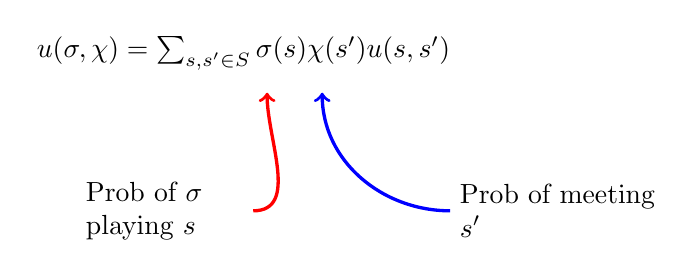
\begin{tikzpicture}
\node (A) at (0,0) {$u(\sigma, \chi)=\sum_{s, s'\in S}\sigma(s)\chi(s')u(s,s')$};
\pause
\node (prob1) at (-1,-2) [text width=2cm] {Prob of $\sigma$ playing $s$};
\draw (prob1) edge[red, very thick, out=0, in=-90, ->] (.3,-.5);

\node (prob2) at (4,-2) [text width=2.5cm] {Prob of meeting $s'$};
\draw (prob2) edge[blue, very thick, out=180, in=-90, ->] (1,-.5);
\end{tikzpicture}
\end{center}
}

\frame{
$$\Huge
\begin{pmatrix}
u(s,s),u(s,s)&u(s,s'),u(s,s')\\
u(s',s),u(s',s) &u(s',s'),u(s',s')\\
\end{pmatrix}
$$
}

\frame{
\textbf{Theorem.}
}

\end{document}
